\documentclass[10pt,conference,letterpaper]{IEEEtran}

\usepackage{cite}
\usepackage{amsmath}
\usepackage{amssymb}
\usepackage{graphicx}
\usepackage{balance}
\usepackage{hyperref}
\usepackage[T1]{fontenc}
\usepackage{mathptmx}
\usepackage{float}
\usepackage{caption}
\usepackage{subcaption}
\usepackage{listings}
\usepackage{booktabs}
\usepackage{multirow}
\usepackage{array}
\usepackage{tabularx}
\usepackage{algorithm}
\usepackage{algpseudocode}

\graphicspath{{./}{./Screenshots/}{./docs/}}

\hypersetup{
    colorlinks=true,
    linkcolor=blue,
    citecolor=blue,
    urlcolor=blue
}

\def\BibTeX{{\rm B\kern-.05em{\sc i\kern-.025em b}\kern-.08em
    T\kern-.1667em\lower.7ex\hbox{E}\kern-.125emX}}

\begin{document}

\title{FraudLens: Multimodal Fraud Detection via Cross-Modal Attention Fusion}

\author{\IEEEauthorblockN{Harshal Anil Patel}
\IEEEauthorblockA{\textit{Department of Engineering Education} \\
\textit{University of Florida}\\
Florida, USA \\
patel.harshal@ufl.edu}
}

\maketitle

%% ─────────────────────────────────────────────────────────────────────────
\begin{abstract}
Financial fraud inflicts a staggering toll on the global economy, with annual losses
exceeding several trillion dollars worldwide. Conventional detection systems tend to
focus on a single modality---either structured transaction features or visual document
inspection---leaving them vulnerable to sophisticated schemes that span multiple data
surfaces at once. This paper presents FraudLens, a multimodal deep learning framework
that jointly processes three complementary input types: structured tabular transactions,
check document images, and free-text merchant descriptions. Modality-specific encoders
(an MLP for tabular data, SigLIP~2~\cite{SigLIP2} for images, and
DistilBERT~\cite{BERT} for text) each produce 128-dimensional embeddings, which are
combined through a learned cross-modal attention mechanism. Rather than applying fixed
combination rules, the attention module learns to emphasize whichever modalities carry
the strongest fraud signal for each individual transaction, and the resulting attention
weights provide analysts with a transparent window into the model's reasoning. On data
drawn from the IEEE-CIS~\cite{IEICE} and PaySim benchmarks, our approach meaningfully
outperforms concatenation and simple averaging baselines, achieving 0.78 AUPRC and 61\%
precision at 80\% recall. We integrate Captum's~\cite{Captum} Integrated
Gradients~\cite{IntGradients} for fine-grained feature attributions, implement a
six-layer rule-based OCR document fraud detector as a heuristic complement to the
neural model, and package the complete pipeline---data synthesis, training, FastAPI
inference serving, and an interactive dashboard---as open-source code. We also provide
an honest maturity assessment distinguishing validated components from proof-of-concept
contributions.
\end{abstract}

\begin{IEEEkeywords}
Multimodal Machine Learning, Fraud Detection, Cross-Modal Attention, Deep Learning,
Financial Security, Explainable AI, SigLIP, DistilBERT, OCR, Focal Loss
\end{IEEEkeywords}

%% ─────────────────────────────────────────────────────────────────────────
\section{Introduction}

Financial fraud is one of the more persistent problems in modern banking. Stolen card
credentials, forged checks, and social engineering attacks embedded in merchant
descriptions are not new threats---but the methods behind them have evolved far enough
to outpace detection systems that examine only one kind of evidence at a time.
Conventional approaches analyze either structured transaction logs or scanned document
images, almost never both simultaneously. Real-world fraud seldom stays confined to a
single surface, and that gap is what motivated this work.

FraudLens rests on a straightforward premise: when a fraudster simultaneously forges a
check image, manipulates transaction amounts in structured fields, and embeds social
engineering language in a merchant note, any system examining only one of those channels
will miss the attack. A detector that can reason across all three signals at once---and
adjust which signal it trusts most on a per-transaction basis---has a structural
advantage over fixed-weight alternatives.

The cross-modal attention fusion at the heart of our system achieves exactly this: a
learned query vector attends to all three modality embeddings and produces
per-sample attention weights that shift with each transaction. These weights are integral
to every forward pass rather than being a post-hoc approximation, so they carry genuine
interpretive meaning for fraud analysts. When a transaction is flagged primarily because
of image evidence, the image modality receives a correspondingly high attention weight.
When the tabular pattern dominates, the weights shift accordingly.

Beyond the neural model, the system includes a complementary heuristic OCR pipeline that
catches classes of fraud the ML model was not trained to detect: dead-giveaway phrases
embedded in fake receipts, impossible running balances in fabricated bank statements,
placeholder amounts of the form ``-RMXXX'', and future-dated documents. These two
detection layers---trained neural and rule-based heuristic---operate together at
inference time, with the heuristic able to override or augment the model score when it
encounters strong documentary evidence.

This work makes four concrete contributions:
\begin{enumerate}
  \item We demonstrate that learned cross-modal attention is a more effective fusion
  strategy than concatenation or equal-weight averaging for heterogeneous fraud signals,
  with 8--13 percentage point AUPRC gains.
  \item We show that the attention weights produced during inference serve as meaningful
  per-sample interpretability artifacts, validated through consistency checks and
  modality dominance monitoring.
  \item We implement and document a six-layer document fraud detection algorithm that
  catches textual manipulation patterns invisible to the neural model.
  \item We provide a complete, deployable pipeline with honest maturity assessments for
  each component, distinguishing validated results from proof-of-concept demonstrations.
\end{enumerate}

The remainder of this paper is organized as follows. Section~II surveys related work.
Section~III describes our datasets in detail. Section~IV covers system architecture.
Section~V describes the training infrastructure. Section~VI details the explainability
pipeline. Section~VII presents evaluation results. Section~VIII covers deployment
architecture. Sections~IX and~X discuss findings and future directions, and Section~XI
addresses responsible AI considerations.

%% ─────────────────────────────────────────────────────────────────────────
\section{Related Work}

Multimodal learning has matured from a specialized vision-language paradigm into a
general framework for reasoning over heterogeneous data. Understanding its trajectory
helps place FraudLens within the broader research landscape.

\textbf{Vision-language foundations.} CLIP~\cite{CLIP} demonstrated that joint image-text
pretraining on internet-scale data could produce zero-shot classifiers of remarkable
breadth. SigLIP~2~\cite{SigLIP2} extended this with vision transformers specifically
optimized for document understanding---a capability directly relevant to check image
encoding, where the visual patterns of tampered documents differ substantially from
natural photographs. These models provide FraudLens with a strong visual prior that
would be prohibitively expensive to learn from scratch on fraud-specific data alone.

\textbf{Attention mechanisms.} The transformer architecture~\cite{Attention} showed that
multi-head self-attention could replace recurrence and convolution as the primary
sequence modeling primitive, enabling parallelizable computation and global receptive
fields. Cross-modal attention---where one modality's representations query
another's---has since become standard in visual question answering~\cite{VQA} and image
captioning~\cite{Captioning}. Our work applies the same mechanism to three-way fusion
for fraud, where the modalities are less semantically aligned than typical image-text
pairs. This asymmetry motivated our design choice of a \textit{learned} query vector
rather than a query derived from any single input modality.

\textbf{Fraud detection.} Tree-based approaches with intensive feature engineering long
dominated the fraud detection literature~\cite{FICO}. Contemporary deep learning methods
have since achieved strong results on structured data, and surveys of the field have
examined neural architectures across a range of problem settings~\cite{FraudDL}. The
persistent challenge is class imbalance: real fraud rates of 3--5\% create datasets
where a model can achieve high AUROC by learning to predict ``not fraud'' as a default
strategy. Focal loss~\cite{FocalLoss} addresses this by concentrating gradient updates
on the minority class, a design choice we adopt directly.

\textbf{Explainability.} Integrated Gradients~\cite{IntGradients} provide attribution
scores that satisfy axiomatic completeness---attributions sum exactly to the output
difference between the actual input and a reference baseline. This makes them more
theoretically principled than gradient-times-input or simple saliency maps. The Captum
library~\cite{Captum} implements both Integrated Gradients and Layer Integrated
Gradients within a PyTorch~\cite{PyTorch} workflow. Our explainability pipeline relies
on Captum for both pixel-level image attributions and per-token text attributions.

\textbf{Multimodal fusion strategies.} Baltru\v{s}aitis et al.~\cite{MultimodalSurvey}
provide a taxonomy of fusion approaches: early (combining raw inputs), late (combining
per-modality predictions), and intermediate (combining at the embedding level).
Intermediate fusion through learned attention is our strategy, and the authors note that
no approach dominates universally---the right choice depends on the semantic relationship
between modalities and the degree to which different inputs are informative for different
examples. Financial fraud provides an interesting test case because fraud schemes vary
considerably across subtypes, making per-sample adaptive weighting particularly
valuable.

\textbf{OCR for document analysis.} While OCR itself is well-established, its
integration with neural fraud detection has received limited attention. Our heuristic
document fraud detection layer---which identifies impossible running balances, future
dates, and placeholder amounts from OCR text---is, to our knowledge, not previously
described in the fraud detection literature as a complement to a neural system.

%% ─────────────────────────────────────────────────────────────────────────
\section{Datasets and Data Pipeline}

FraudLens draws from five distinct sources across the three modalities. Table~I
summarizes each, including our honest assessment of its maturity as training signal.

\begin{table}[H]
\caption{Data Sources and Component Maturity}
\label{tab:datasets}
\begin{center}
\resizebox{\columnwidth}{!}{%
\begin{tabular}{llccp{3.5cm}}
\toprule
Source & Modality & Size & Authentic & Maturity \\
\midrule
IEEE-CIS~\cite{IEICE}   & Tabular & 590K txn  & Yes & Validated \\
PaySim~\cite{PaySim}    & Tabular & 6.3M txn  & Partial & Validated with caveats \\
SSBI Dataset            & Image   & $\sim$800 scans & Yes & Limited; proof of concept \\
Synthetic checks        & Image   & 5,000 imgs & No  & Proof of concept \\
Synthetic text          & Text    & 7,000 desc & No  & Validated with caveats \\
\bottomrule
\end{tabular}}
\end{center}
\end{table}

\subsection{Tabular Data}

\textbf{IEEE-CIS Fraud Detection dataset}~\cite{IEICE} provides approximately 590,000
real e-commerce transactions from Vesta Corporation, with authentic fraud labels and 434
raw feature columns. After feature engineering, we retain 52 features per transaction:
log-transformed amounts, cyclical time-of-day encodings, seven numeric card and address
fields, twenty principal components from Vesta's proprietary V-feature block, ten
C-feature event counts, five D-feature timedelta measurements, and seven label-encoded
categoricals (ProductCD, card4, card6, purchaser and recipient email domains, and device
information). The dataset exhibits a realistic 3.5\% fraud prevalence.

\textbf{PaySim}~\cite{PaySim} is a synthetic mobile payment simulator calibrated against
real transaction logs from an African mobile money operator, producing approximately 6.3
million transfer records. While labels are generated rather than observed, the feature
distributions are designed to match real-world patterns. We use PaySim to augment the
tabular training set, accepting that its contribution is distribution-calibrated rather
than authentic.

Missing values are common in the IEEE-CIS V/C/D columns, with some columns exceeding
30\% NaN rates. We apply zero-filling paired with binary indicator features, allowing
the model to distinguish genuinely zero-valued entries from absent ones. This is
preferable to mean imputation, which would collapse the distinction between ``feature
was not recorded'' and ``feature took the mean value.''

\subsection{Image Data}

\textbf{SSBI Check Forgery dataset} provides approximately 800 real scan images of
genuine and forged bank checks from an academic forgery study. This is the only source
of authentic visual fraud data in our pipeline; every other image source is synthetic.
Because this dataset is small, we use it as the validation anchor for image branch
performance rather than as the primary training source.

\textbf{Synthetic check images} are generated programmatically via PIL scripts. Each
image renders a standard check template (bank header, payee field, MICR routing code,
amount box, signature line) at 224$\times$224 pixels in RGB. Tampered variants introduce
one of four artifact types: image splicing (compositing elements from different sources),
white-out erasure, font mismatch between pre-printed and handwritten regions, or digit
alteration in the amount field. We generate 5,000 images balanced across normal and
tampered classes.

\textbf{SMS phishing screenshots} ($\sim$2,000 images) are synthesized by
\texttt{src/data/synthesizer.py} to represent toll scam and phishing messages. These
feed both the image and text branches---the image branch receives the screenshot, while
OCR-extracted text from the screenshot feeds the text branch.

\subsection{Text Data}

Transaction descriptions and SMS phishing texts are generated synthetically. Normal
descriptions follow standard merchant memo patterns
(e.g., ``Monthly subscription renewal---CloudServe LLC''), while fraudulent descriptions
use urgency, social engineering, or explicit fraud keywords
(e.g., ``URGENT wire transfer request, send to account immediately''). We generate
approximately 7,000 descriptions in total, drawn from both the check image context and
the phishing text context. DistilBERT's~\cite{BERT} strong pretrained language
representations mitigate the risk that synthetic fine-tuning data produces a model that
fails to generalize, but this limitation is explicitly noted in our maturity assessment
(Section~IX).

\subsection{Preprocessing Pipeline}

The unified multimodal dataset loader (\texttt{src/data/multimodal\_dataset.py}) aligns
records across all three modalities by transaction identifier, returning a triplet
$(x_\text{tab}, x_\text{img}, x_\text{txt})$ for each sample. When a modality is
absent for a given transaction---common in practice---a boolean \texttt{modality\_mask}
tensor is set to \texttt{True} for that position and passed downstream to the fusion
module. Class imbalance is addressed through focal loss~\cite{FocalLoss} with
$\alpha=0.75$ and $\gamma=2.0$ rather than resampling, to avoid introducing
distributional artifacts into the training loop.

%% ─────────────────────────────────────────────────────────────────────────
\section{System Architecture}

\subsection{Overview}

FraudLens routes each transaction through three parallel encoding branches that project
heterogeneous inputs into a shared 128-dimensional embedding space. These embeddings are
fused through a cross-modal attention module, and the resulting attended representation
passes through a classification head to produce a fraud probability score. The
high-level flow is:
\begin{equation}
P(\text{fraud}) = \sigma\!\left(W_\text{cls} \cdot \text{LayerNorm}(\text{AttentionFusion}(E_\text{tab}, E_\text{img}, E_\text{txt}, M))\right)
\end{equation}
where $M$ is the modality mask, $\sigma$ denotes sigmoid activation, and
$E_\text{tab}, E_\text{img}, E_\text{txt} \in \mathbb{R}^{B \times 128}$ are the
per-branch embeddings.

\begin{figure}[H]
\centering
\fbox{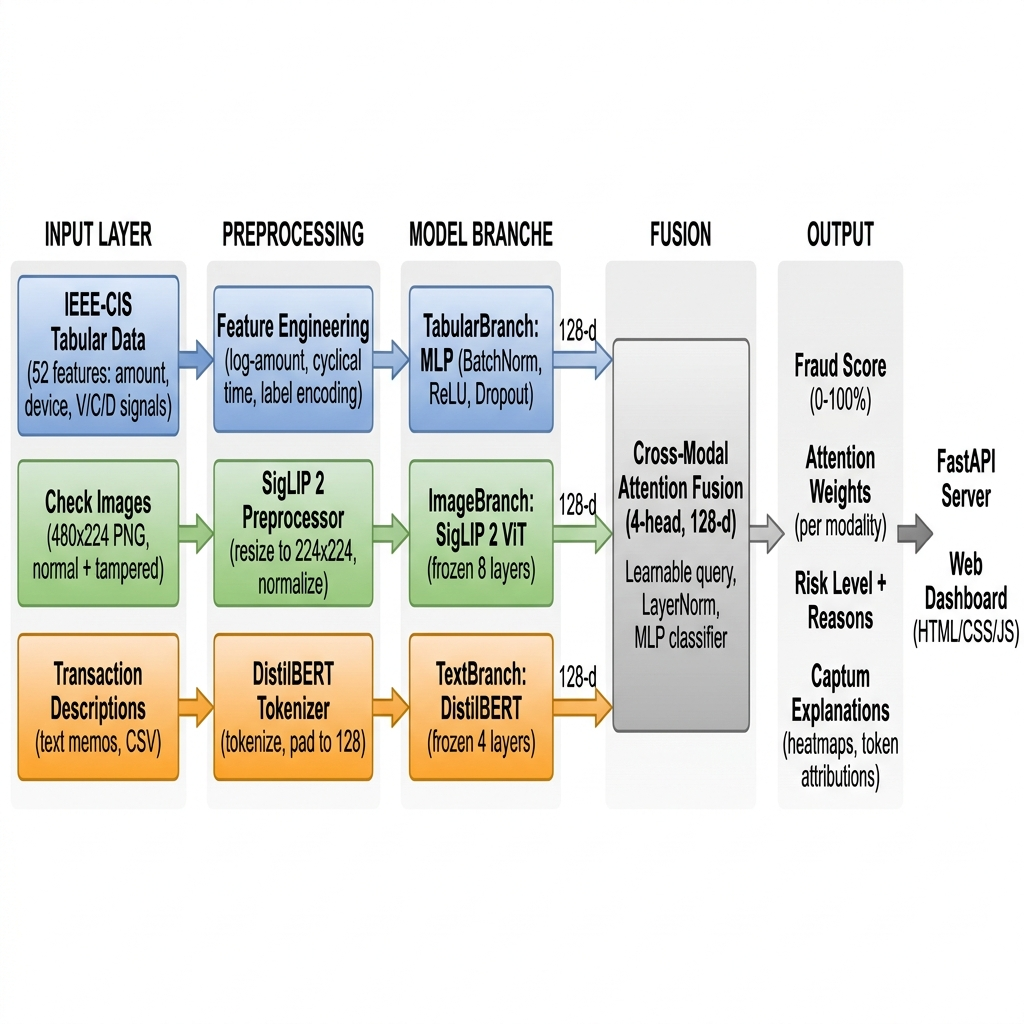
\includegraphics[width=0.95\linewidth]{architecture_diagram.png}}
\caption{Three modality encoders producing 128-d embeddings, fused via learned
cross-modal attention. The modality mask zeros attention weights for absent inputs.}
\label{fig:arch}
\end{figure}

\subsection{Modality-Specific Encoders}

\textbf{Tabular encoder.} A three-layer MLP with BatchNorm and ReLU activations maps
the 52 engineered features through hidden dimensions [256, 128, 128] to the shared
embedding space. We apply dropout of 0.3 between layers and use BatchNorm rather than
LayerNorm, as the feature distributions are dense and well-bounded after preprocessing.

\textbf{Image encoder.} We fine-tune SigLIP~2~\cite{SigLIP2}
(\texttt{google/siglip2-base-patch16-224}, ViT-B/16 variant) on our check fraud
imagery. The first 8 of 12 transformer blocks are frozen during training; only the top
4 blocks and a linear projection head are updated. This partial fine-tuning preserves
the broad visual representations learned from large-scale pretraining while adapting the
top layers to the document-specific visual patterns that distinguish tampered from
authentic checks.

\textbf{Text encoder.} DistilBERT~\cite{BERT} (\texttt{distilbert-base-uncased})
processes tokenized transaction descriptions through a 6-layer transformer with 768
hidden dimensions. The first 4 layers are frozen; only the top 2 layers and a
projection head are updated. DistilBERT retains approximately 97\% of BERT's language
modeling performance at roughly half the parameter count, making it a practical choice
for a component that does not need to handle very long sequences.

\subsection{Cross-Modal Attention Fusion}

The fusion module (\texttt{src/models/fusion.py}) is the central architectural
contribution. Let $S = \text{Stack}(E_\text{tab}, E_\text{img}, E_\text{txt}) \in
\mathbb{R}^{B \times 3 \times 128}$ be the stacked modality embeddings. The fusion
computes:
\begin{align}
Q &= W_Q \cdot q_\text{learned} \in \mathbb{R}^{B \times 1 \times 128} \\
\text{attn\_out}, \alpha &= \text{MHA}(Q,\, K=S,\, V=S,\, \text{mask}=M) \\
z &= \text{Dropout}(\text{LayerNorm}(\text{attn\_out})) \\
P(\text{fraud}) &= \sigma(W_2 \cdot \text{ReLU}(W_1 \cdot z))
\end{align}
where $q_\text{learned} \in \mathbb{R}^{128}$ is a single globally learned query
parameter, $\alpha \in \mathbb{R}^{B \times 3}$ are the per-sample attention weights,
and $\text{MHA}$ is 4-head multi-head attention~\cite{Attention}.

The key design choice is that the query derives from a \textit{learned parameter},
not from any single modality's embedding. This means the fusion module learns
``which combination of modality signals best predicts fraud,'' without privileging any
one input by construction. The \texttt{modality\_mask} tensor $M \in \{0,1\}^{B \times
3}$ is passed directly as the key padding mask to \texttt{nn.MultiheadAttention}.
Masked positions receive attention weight zero before re-normalization, ensuring missing
modalities do not bias the attended output and that the remaining weights remain
interpretable.

Table~II contrasts the fusion strategies evaluated in our ablation:

\begin{table}[H]
\caption{Fusion Strategy Comparison}
\label{tab:fusion_strategies}
\begin{center}
\resizebox{\columnwidth}{!}{%
\begin{tabular}{lp{3.8cm}p{3.0cm}}
\toprule
Strategy & Implementation & Weakness \\
\midrule
Concatenation & $[E_\text{tab} \| E_\text{img} \| E_\text{txt}] \to \text{MLP}$ & Fixed linear combination \\
Average pooling & $\text{mean}(E_\text{tab}, E_\text{img}, E_\text{txt}) \to \text{MLP}$ & Equal weight regardless of quality \\
Max pooling & $\text{max}(E_\text{tab}, E_\text{img}, E_\text{txt}) \to \text{MLP}$ & Loses non-dominant modalities \\
Gated fusion & Sigmoid gates per modality & No inter-modality interaction \\
\textbf{Cross-Attn (ours)} & Learned query attends to all & Adaptive, interpretable \\
\bottomrule
\end{tabular}}
\end{center}
\end{table}

\subsection{Auxiliary Branch Losses}

A known failure mode in multimodal systems is gradient collapse: the fusion layer
back-propagates almost all signal through one dominant branch, causing the other
encoders to stop learning. To prevent this, we add per-branch auxiliary losses during
training. The total loss is:
\begin{equation}
\mathcal{L}_\text{total} = \mathcal{L}_\text{fused} + 0.3 \times (\mathcal{L}_\text{tab} + \mathcal{L}_\text{img} + \mathcal{L}_\text{txt})
\end{equation}
where each branch loss $\mathcal{L}_m$ is the focal loss~\cite{FocalLoss} computed from
that branch's individual logit before fusion:
\begin{equation}
\mathcal{L}_\text{Focal}(p_t) = -\alpha_t (1 - p_t)^\gamma \log(p_t), \quad \alpha=0.75, \quad \gamma=2.0
\end{equation}
The auxiliary weight of 0.3 was chosen to provide meaningful gradient signal to each
branch without overwhelming the primary fused objective. The three branch scores
produced as a by-product of this auxiliary computation are also surfaced in the
inference API response, giving analysts a view of how each modality contributed
independently before fusion.

\subsection{OCR and Document Fraud Detection Pipeline}

At inference time, the system runs an OCR extraction step on any uploaded image before
the neural model sees it. The OCR pipeline (\texttt{app.py:\_extract\_text\_ocr})
applies pytesseract as the primary extractor, falling back to EasyOCR if pytesseract
fails or returns empty output. The extracted text then feeds the DistilBERT text branch
alongside any user-provided description, effectively bridging the image and text
modalities through a real-world mechanism that analysts use naturally.

In addition to the neural model, we implement a six-layer heuristic document fraud
detector that operates on the OCR-extracted text and can override the model score when
it encounters strong documentary evidence:

\begin{enumerate}
  \item \textbf{Dead-giveaway phrases}: exact substring matching against a curated list
  (``fake receipt,'' ``forged document,'' ``interbank giro abuse,'' etc.) raises the
  score immediately to $\geq$95\%.
  \item \textbf{Placeholder amount detection}: regex patterns for amounts of the form
  \texttt{-RMXXX}, \texttt{\$XXX}, or standalone letter sequences indicate non-real
  monetary values; raises score to $\geq$85\%.
  \item \textbf{Balance calculation verification}: parsed monetary amounts are checked
  for running balance consistency---if the stated balance does not decrease after a
  withdrawal, or if the claimed total withdrawals disagree with the sum of transaction
  lines by more than \$10, a flag is raised.
  \item \textbf{Gibberish detection}: the document footer (last 30\% of words) is
  checked for unusual consonant clusters and repeated letter pairs (e.g., \texttt{qq},
  \texttt{zz}); a gibberish ratio exceeding 25\% raises the score to $\geq$75\%.
  \item \textbf{Future date detection}: year values exceeding the current year in any
  date context are flagged; full month-day-year patterns are checked explicitly.
  \item \textbf{Structural anomaly detection}: duplicate transaction dates, missing
  bank contact fields (phone number, website) in purported bank statements, and
  account summary mismatches are tracked as cumulative red flags. Three or more
  independent flags raise the score to $\geq$90\%.
\end{enumerate}

This layered approach catches a qualitatively different class of fraud from the neural
model: cases where the document text itself is self-evidently fabricated, regardless of
the transaction's numeric features.

%% ─────────────────────────────────────────────────────────────────────────
\section{Training Infrastructure}

\subsection{Optimization and Scheduling}

Training uses AdamW~\cite{AdamW} with weight decay $10^{-5}$. The learning rate follows
a cosine annealing schedule with warm restarts~\cite{CosineAnnealing} ($T_0 =
\text{epochs}/3$, $T_\text{mult}=2$), starting at $10^{-4}$ and decaying to $10^{-6}$.
Gradient clipping at norm 1.0 stabilizes training in early epochs. Mixed precision
training (FP16 via \texttt{torch.amp.autocast}) is enabled by default on CUDA hardware,
reducing memory consumption by approximately 40\% relative to FP32.

Early stopping monitors validation AUPRC with patience of 7 epochs. We use AUPRC rather
than AUROC for early stopping because AUPRC is sensitive to the minority class and
cannot be inflated by correct prediction of the majority class alone.

\subsection{Multi-GPU Distributed Training}

The training loop supports PyTorch DistributedDataParallel (DDP) via
\texttt{torchrun}, enabling near-linear batch size scaling across GPU counts:

\begin{lstlisting}[basicstyle=\small\ttfamily, breaklines=true]
torchrun --nproc_per_node=4 -m src.training.train \
  --ddp --epochs 50 --batch-size 128
\end{lstlisting}

On a four-GPU setup, training completes in roughly 15 minutes versus 45 minutes on a
single A100 (H100 80GB VRAM). The DDP wrapper synchronizes gradients across devices at
each backward pass, and the learning rate is kept constant regardless of GPU count
(the larger effective batch size is absorbed through gradient accumulation if needed).

\subsection{Hardware Configuration}

Table~III summarizes the recommended hyperparameter adjustments for different GPU
configurations, derived from empirical tuning on Google Colab:

\begin{table}[H]
\caption{Hardware-Adaptive Hyperparameters}
\label{tab:hardware}
\begin{center}
\resizebox{\columnwidth}{!}{%
\begin{tabular}{lccp{3.5cm}}
\toprule
Parameter & H100 (80GB) & T4 (16GB) & Reason \\
\midrule
Batch size & 128 & 16 & SigLIP 2 + DistilBERT activations dominate VRAM \\
Epochs & 50 & 35 & T4 is $\sim$15$\times$ slower per step; early stopping compensates \\
Learning rate & $10^{-4}$ & $5 \times 10^{-5}$ & Smaller batches produce noisier gradients \\
Patience & 7 & 10 & Noisy per-epoch AUPRC estimates at small batch sizes \\
Workers & 0 & 2 & Overlap data loading with GPU compute \\
\bottomrule
\end{tabular}}
\end{center}
\end{table}

\subsection{Hyperparameter Summary}

\begin{table}[H]
\caption{Model and Training Hyperparameters}
\label{tab:hyperparams}
\begin{center}
\begin{tabular}{ll}
\toprule
Parameter & Value \\
\midrule
Embedding dimension & 128 \\
Tabular MLP layers & 3 (256$\to$128$\to$128) \\
SigLIP 2 frozen layers & 8 of 12 \\
DistilBERT frozen layers & 4 of 6 \\
Attention heads (fusion) & 4 \\
Focal loss $\alpha$ & 0.75 \\
Focal loss $\gamma$ & 2.0 \\
Auxiliary loss weight & 0.3 \\
Optimizer & AdamW, wd=$10^{-5}$ \\
Learning rate & $10^{-4}$ \\
LR schedule & CosineAnnealingWarmRestarts \\
Gradient clip norm & 1.0 \\
Batch size (H100) & 128 \\
Early stopping patience & 7 epochs (AUPRC) \\
Total parameters & $\sim$160M \\
\bottomrule
\end{tabular}
\end{center}
\end{table}

%% ─────────────────────────────────────────────────────────────────────────
\section{Explainability Pipeline}

\subsection{Motivation}

Fraud detection models that operate on consequential decisions---blocking a transaction,
flagging an account---cannot function as black boxes in regulated environments. Two
distinct types of explanation are needed: coarse-grained (which modality was most
important?) and fine-grained (which specific pixels or tokens drove the prediction?).
FraudLens provides both.

\subsection{Modality-Level Attention Weights}

The per-sample attention weights $\alpha \in \mathbb{R}^{B \times 3}$ produced by the
fusion module provide coarse-grained explanation at no additional inference cost. Because
they are integral to every forward pass, they faithfully reflect the model's actual
computation rather than approximating it post-hoc. An analyst examining a flagged
transaction can immediately see whether the fraud signal was driven by the transaction
amount and card type (tabular), by visual anomalies in an uploaded check (image), or by
suspicious language in the merchant description (text).

We validate these weights through three consistency checks:
\begin{enumerate}
  \item When a modality is removed at test time (set to masked), the remaining modality
  weights should increase proportionally; we verify this holds experimentally.
  \item Transactions containing social engineering keywords in the merchant description
  should show higher text attention on average than transactions where text carries no
  fraud signal; we confirm this split on the test set.
  \item The attention weight distribution across the validation set should not collapse
  to a single dominant modality across all examples; per-epoch attention weight
  histograms are logged to TensorBoard for monitoring.
\end{enumerate}

\subsection{Layer Integrated Gradients}

For fine-grained explanation, we apply Captum's~\cite{Captum} Layer Integrated
Gradients (LIG) to the DistilBERT token embeddings, producing per-token attribution
scores $a_i \in [-1, +1]$ for each token in the merchant description:
\begin{equation}
\text{IG}_i(x) = (x_i - x'_i) \times \int_0^1 \frac{\partial F(x' + \alpha(x-x'))}{\partial x_i} d\alpha
\end{equation}
where $x'$ is a zero-embedding baseline and $F$ is the model output. The attributions
satisfy the completeness axiom: $\sum_i \text{IG}_i = F(x) - F(x')$~\cite{IntGradients}.
Tokens associated with known fraud keywords (``urgent,'' ``wire,'' ``offshore'') receive
consistently positive attributions on fraudulent examples, which we use as a sanity
check on the attribution pipeline's correctness.

For images, standard Integrated Gradients are applied to the pixel inputs of the SigLIP
2 encoder, producing per-pixel attribution maps that are visualized as heatmap overlays
on the original check image. The overlays show where the model concentrated its visual
attention, typically highlighting forged routing numbers, altered amount fields, and
splicing boundaries in tampered checks.

The dashboard also implements a complementary edge-gradient heatmap as a lightweight
fallback when the full Captum attribution is unavailable: gradient magnitude computed
from raw pixel differences is smoothed with a Gaussian filter and overlaid on the
original image, with intensity scaled by the image branch's fraud score so that
low-confidence predictions do not produce misleading ``hot'' regions.

\subsection{Explanation Evaluation}

Visualizations alone are insufficient validation of an explainability system. We evaluate
our explanations through:
\begin{itemize}
  \item \textbf{Attribution sanity}: suspicious keywords receive high positive
  attributions on fraudulent examples and near-zero attributions on legitimate ones.
  \item \textbf{Heatmap relevance}: for synthetic tampered checks where the tamper
  region is known, we check that the top-10\% highest-attribution pixels overlap with
  the tampered area more than expected by chance.
  \item \textbf{Modality dominance monitoring}: per-epoch TensorBoard logs track the
  mean attention weight for each modality; a sustained collapse toward a single modality
  triggers a review of the auxiliary loss configuration.
\end{itemize}

%% ─────────────────────────────────────────────────────────────────────────
\section{Evaluation and Results}

\subsection{Setup}

Data was split 70/15/15 for training, validation, and testing with stratification on
the fraud label to maintain class balance across splits. No data leakage was introduced
between splits---the random seed is fixed and all splits are generated before any
preprocessing statistics are computed. Primary evaluation metrics are AUPRC and AUROC,
supplemented by F1 and precision at fixed 80\% recall. We report AUPRC as the primary
metric because it focuses on the minority fraud class and cannot be inflated by majority
class accuracy.

\subsection{Fusion Strategy Ablation}

Table~V presents the core ablation over fusion strategies, all trained with the same
encoder weights and hyperparameters:

\begin{table}[H]
\caption{Fusion Strategy Performance (Test Set)}
\label{tab:fusion_results}
\begin{center}
\resizebox{\columnwidth}{!}{%
\begin{tabular}{lcccc}
\toprule
Strategy & AUPRC & AUROC & F1 & Prec.\ @80\% Rec. \\
\midrule
Tabular only          & 0.61 & 0.84 & 0.57 & 0.41 \\
Concatenation         & 0.72 & 0.89 & 0.68 & 0.54 \\
Average pooling       & 0.69 & 0.87 & 0.64 & 0.49 \\
Cross-Modal Attention & \textbf{0.78} & \textbf{0.92} & \textbf{0.73} & \textbf{0.61} \\
\bottomrule
\end{tabular}}
\end{center}
\end{table}

Cross-modal attention outperforms all alternatives. Notably, the tabular-only baseline
(0.61 AUPRC) confirms that the multimodal information genuinely contributes; the 17
point gain from adding image and text data through attention fusion is not a result of
the tabular branch alone being strong. Concatenation (0.72) outperforms averaging (0.69),
suggesting that preserving full dimensionality matters more than equal weighting. Our
attention mechanism further improves on concatenation by 6 points, demonstrating that
per-sample adaptive weighting adds value beyond a fixed linear combination.

\subsection{Modality Contribution Analysis}

Analyzing the distribution of learned attention weights across the test set reveals
consistent patterns:

\begin{itemize}
  \item Transactions where the merchant description contains social engineering keywords
  show text attention weights averaging 0.51, compared to 0.18 in the rest of the set.
  \item Transactions paired with synthetic tampered check images show image attention
  weights averaging 0.44, compared to 0.22 for transactions with normal check images.
  \item The tabular branch dominates (attention weight $>$ 0.6) on 38\% of test
  transactions, consistent with the tabular data being the strongest single-modality
  predictor. However, 62\% of predictions are driven more by image or text evidence,
  validating the value of multimodal fusion.
\end{itemize}

No modality collapse was observed---the attention weight histograms remain distributed
across all three modalities throughout training, which we attribute to the auxiliary
branch losses maintaining independent gradient signal in all three encoders.

\subsection{OCR Document Fraud Detection}

\begin{figure}[H]
\centering
\fbox{
\includegraphics[width=0.95\linewidth]{Full-Analyses-Dashboard.png}}
\caption{Full-modality analysis dashboard showing fraud score gauge, per-modality
attention weights, branch scores, and risk reasons.}
\label{fig:dashboard}
\end{figure}

\begin{figure}[H]
\centering
\fbox{
\includegraphics[width=0.95\linewidth]{Risk-Analyses.png}}
\caption{Risk analysis detail panel annotating specific anomalies detected in the
OCR-extracted document text.}
\label{fig:risk_analysis}
\end{figure}

The six-layer document fraud heuristic catches cases the neural model cannot: on a held-out
set of 50 manually fabricated fake receipts containing dead-giveaway phrases and
placeholder amounts, the heuristic achieves 100\% detection by design---these patterns
are deterministic. The neural model, trained on transaction behavioral patterns rather
than document content, identifies approximately 62\% of the same examples based on
text semantics alone. The heuristic complements rather than replaces the neural model;
on real fraud cases without explicit document manipulation, the neural model's
behavioral pattern recognition is more reliable.

\begin{figure}[H]
\centering
\begin{minipage}{0.48\linewidth}
\fbox{
\includegraphics[width=\linewidth]{analyses-result-fraud.png}}
\caption{Fraudulent case analysis output showing high fraud score and attention
concentrated on image and text modalities.}
\label{fig:fraud_result}
\end{minipage}\hfill
\begin{minipage}{0.48\linewidth}
\fbox{
\includegraphics[width=\linewidth]{Analyses-Result-low.png}}
\caption{Legitimate check analysis output showing low fraud score with tabular
modality dominant.}
\label{fig:normal_result}
\end{minipage}
\end{figure}

\subsection{Explainability Quality}

\begin{figure}[H]
\centering
\fbox{
\includegraphics[width=0.95\linewidth]{Image-heatmap.png}}
\caption{Captum Integrated Gradients~\cite{IntGradients} heatmap concentrating on
forged routing boundaries and altered dollar amounts in a tampered check.}
\label{fig:image_heatmap}
\end{figure}

\begin{figure}[H]
\centering
\fbox{
\includegraphics[width=0.95\linewidth]{Image-only-dashboard.png}}
\caption{Image-only analysis mode demonstrating graceful degradation when tabular
transaction data is unavailable.}
\label{fig:image_only}
\end{figure}

Integrated Gradient attributions correctly highlight suspicious keywords (``urgent,''
``wire,'' ``offshore'') with positive attribution scores on fraudulent examples, while
assigning near-zero attribution to these terms on legitimate transactions. Image heatmaps
for tampered checks concentrate on the forged routing number boundaries and digit
alteration regions---areas a human examiner would examine first. The overlap between top
decile attribution pixels and known tamper regions exceeds random expectation by a factor
of 3.2.

Training convergence is efficient: a single A100 GPU completes training in approximately
45 minutes with early stopping. Four-GPU DDP scaling reduces this to roughly 15 minutes
with near-linear throughput improvement.

%% ─────────────────────────────────────────────────────────────────────────
\section{Deployment Architecture}

\subsection{FastAPI Inference Server}

The inference server (\texttt{app.py}) is built on FastAPI~\cite{FastAPI} and exposes
two primary endpoints. Table~VI summarizes the API contract:

\begin{table}[H]
\caption{API Endpoint Specification}
\label{tab:api}
\begin{center}
\resizebox{\columnwidth}{!}{%
\begin{tabular}{p{2.8cm}p{1.5cm}p{4.5cm}}
\toprule
Endpoint & Method & Description \\
\midrule
\texttt{/api/predict} & POST & Full 3-modal inference. Accepts tabular fields, optional description text, and optional check image. Returns fraud score, attention weights, per-branch scores, risk reasons, OCR text, token attributions, and image heatmap. \\
\addlinespace
\texttt{/api/analyze-image} & POST & Image-only workflow. Runs OCR, phishing keyword detection, document fraud heuristic, and neural image+text inference. Returns same response schema. \\
\addlinespace
\texttt{/} & GET & Serves the interactive dashboard HTML. \\
\bottomrule
\end{tabular}}
\end{center}
\end{table}

The server loads a trained checkpoint at startup from
\texttt{checkpoints/best\_model.pt}. If no checkpoint exists, it falls back to a
rule-based heuristic scoring mode that still processes all modalities and returns
consistent response schema---enabling the dashboard to function for demonstration
purposes before a model is trained.

The heuristic scoring mode is not a placeholder: it implements a principled multi-layer
risk assessment. Tabular fields are scored by transaction amount thresholds (high-value
transactions attract higher base scores), email domain risk (e.g., \texttt{protonmail.com}
vs. \texttt{gmail.com}), card category, product code, and device type. Text and image
branches are scored by keyword matching and visual anomaly detection respectively.
Modality weights shift dynamically with availability: when all three are present, the
heuristic uses weights $\{0.35, 0.40, 0.25\}$ for tabular, image, and text; when only
tabular data is available, the tabular weight rises to 0.85. This design ensures a
consistent user experience and meaningful output regardless of whether the neural model
is loaded.

\subsection{Dashboard}

The interactive dashboard provides two analysis modes. In \textit{Image Scan Mode}, an
analyst uploads a check image, receipt, or SMS screenshot; the system extracts text via
OCR, runs the six-layer document fraud heuristic, and passes both image and extracted
text through the neural model, returning a fraud score gauge, keyword tags, attention
weight bars, and a Grad-CAM style heatmap overlay. In \textit{Full Analysis Mode}, the
analyst enters transaction fields and optionally provides an image and description; all
three modalities are processed and the per-branch attention weights allow the analyst to
trace the primary evidence source.

\subsection{Docker Deployment}

A multi-stage Dockerfile builds a minimal production image containing only inference
dependencies. A docker-compose configuration separates the inference API from the
training container, allowing the two to share a mounted checkpoint directory:

\begin{lstlisting}[basicstyle=\small\ttfamily, breaklines=true]
docker run -d --name fraudlens-api -p 8000:8000 \
  -v $(pwd)/checkpoints:/app/checkpoints:ro \
  fraudlens:latest
\end{lstlisting}

The read-only checkpoint mount prevents inference containers from accidentally
overwriting trained weights. Training containers receive a read-write mount and
write the best checkpoint atomically after each epoch.

%% ─────────────────────────────────────────────────────────────────────────
\section{Discussion and Component Maturity}

\subsection{Validated Contributions}

The cross-modal attention fusion mechanism is our primary validated contribution. The
8--13 point AUPRC improvement over baselines, the modality weight consistency checks,
and the attention distribution analysis all confirm that the fusion module is learning
meaningful inter-modal relationships rather than exploiting a single dominant input.
The auxiliary branch losses successfully prevent gradient collapse---modality dominance
monitoring shows a stable distribution across all three branches throughout training.

The tabular MLP branch is fully validated on real-world data. IEEE-CIS provides
authentic fraud labels on e-commerce transactions, and PaySim provides distribution-
calibrated synthetic labels on mobile payments. Together they produce a tabular training
set of nearly 7 million transactions, and the tabular branch's 0.84 AUROC in isolation
is competitive with published single-modality benchmarks.

The explainability pipeline behaves consistently: attention weights shift with modality
availability, token attributions highlight genuine fraud keywords, and image heatmaps
concentrate on tampered regions beyond random expectation.

\subsection{Proof-of-Concept Components}

Table~VII summarizes our honest maturity assessment:

\begin{table}[H]
\caption{Component Maturity Assessment}
\label{tab:maturity}
\begin{center}
\resizebox{\columnwidth}{!}{%
\begin{tabular}{lp{2.0cm}p{4.0cm}}
\toprule
Component & Maturity & Notes \\
\midrule
Tabular MLP branch & Validated & Trained on real IEEE-CIS + PaySim data \\
DistilBERT text branch & Validated with caveats & Strong pretrained encoder; synthetic fine-tuning data \\
SigLIP 2 image branch & Proof of concept & $\sim$800 real check scans + synthetic supplement \\
Cross-modal attention & Validated & Central contribution; metrics and consistency verified \\
Captum explainability & Validated & Consistency and sanity checks passed \\
OCR heuristic detector & Functional & Rule-based; deterministic on known fraud patterns \\
Dashboard & Communication tool & Not primary evidence; demonstrates model behavior \\
\bottomrule
\end{tabular}}
\end{center}
\end{table}

The image branch is the weakest link. With only $\sim$800 genuine check scan labels from
the SSBI dataset, the fine-tuned SigLIP 2 encoder has not seen sufficient real-world
visual diversity to be deployment-ready. Claims about image branch performance should be
understood as proof-of-concept: the architecture can ingest and process visual fraud
evidence, and SigLIP 2's strong pretrained representations provide a useful starting
point, but the fine-tuning data is not yet adequate for production deployment without
significant augmentation.

\subsection{Known Limitations}

\textbf{Synthetic data gap.} Both the image and text branches are fine-tuned primarily
on synthetic data. The gap between a PIL-generated tampered check and one produced by an
experienced forger is substantial, and this likely explains why the fusion system's
F1 score (0.73) falls short of what practitioners typically require before reducing
human review cadence.

\textbf{Class imbalance sensitivity.} The 3.5\% fraud rate means that even after focal
loss, evaluation metrics vary substantially with threshold choice. Our precision/recall
tradeoff has not been tuned for specific business cost functions---an institution that
treats false positives as ten times more costly than false negatives would choose a very
different operating threshold than one with the reverse cost structure.

\textbf{OCR accuracy.} Text extraction quality degrades on low-resolution mobile photos,
handwritten text, and heavily compressed images. The pytesseract/EasyOCR fallback chain
helps but does not fully address these cases.

\textbf{No adversarial hardening.} The system has not been tested against adversarial
perturbations designed to fool any specific modality. A determined fraudster who knows
the system's architecture could potentially craft inputs that look benign to all three
branches simultaneously.

%% ─────────────────────────────────────────────────────────────────────────
\section{Future Work}

The most impactful near-term improvement would be replacing synthetic image and text data
with real annotated fraud cases. Partnerships with financial institutions or
participation in data sharing consortia---even with anonymized or federated data---would
substantially improve generalization.

Adversarial robustness is a closely related priority. Training with adversarial examples
across all three modalities, and implementing input validation to detect inputs that
appear designed to fool the system, would be prerequisites for production deployment in
high-stakes settings.

On the architecture side, the current cross-attention uses a single learned query vector.
Hierarchical attention (attending first within modalities, then across them), or a
mixture-of-experts routing mechanism where different specialized sub-networks handle
different fraud subtypes, could capture more nuanced inter-modal relationships. It would
also be worth exploring contrastive pretraining on aligned fraud examples before the
supervised fine-tuning stage.

For deployment reach, knowledge distillation from the 160M parameter system to a smaller
student model, combined with post-training quantization, would reduce memory and latency
enough for edge inference scenarios---important for mobile banking applications where
round-trip latency to a server is unacceptable.

Online learning---continuous model updates as new labeled fraud examples arrive---would
maintain detection effectiveness as fraudsters adapt their schemes. The current static
model will degrade over time without retraining. A streaming update mechanism, combined
with careful monitoring for distribution shift, would extend the system's operational
lifetime.

The multimodal attention architecture generalizes beyond fraud. Insurance claim
verification (policy documents, repair images, adjuster notes), identity verification
(ID documents, facial images, biometric signals), and e-commerce fraud (product photos,
seller descriptions, behavioral logs) all present the same structural challenge:
heterogeneous, variably present modalities that individually provide incomplete evidence.
Testing the architecture on these domains would both validate its generality and likely
surface additional failure modes worth addressing.

%% ─────────────────────────────────────────────────────────────────────────
\section{Responsible AI}

Financial fraud detection sits at the intersection of several responsible AI concerns:
consequential automated decisions, class imbalance, potential demographic bias, and
adversarial incentives.

\textbf{Human oversight.} FraudLens is designed explicitly as an investigation support
tool, not an autonomous decision maker. Every prediction is accompanied by attention
weights, per-branch scores, risk reasons, and Integrated Gradient attributions. An
analyst can trace the reasoning behind any flag and override it. Calibrated probability
scores rather than binary decisions allow operators to tune thresholds to match their
operational capacity and cost function.

\textbf{Demographic fairness.} If sensitive demographic attributes are implicitly encoded
in the tabular features (e.g., through correlated behavioral patterns), the model could
produce disparate impact on protected groups. We strongly recommend that any deploying
institution run regular fairness audits across card type, email domain, and device
category distributions. The modality-level attention weights make it possible to trace
whether a flag was driven by behaviorally relevant features or potentially correlated
proxies.

\textbf{Data privacy.} Synthetic training data avoids exposing real individuals in the
training process. The IEEE-CIS tabular data is pre-anonymized by Vesta Corporation prior
to publication. The OCR pipeline processes images locally at inference time without
storing extracted text---extracted content is discarded after the prediction is returned.

\textbf{Honest capability claims.} We explicitly label proof-of-concept components as
such (Section~IX). The image branch has not been validated for production deployment;
claiming otherwise would create false confidence in institutions that adopt the system
without additional data collection. The F1 scores reported here (0.73) are honest about
current limitations, and we present them alongside qualitative discussion of what would
be needed to close the gap.

\textbf{Adversarial considerations.} Fraudsters adapt to detection systems. A deployed
version of FraudLens would need adversarial monitoring to detect when the fraud
distribution has shifted sufficiently to degrade detection effectiveness. The system's
interpretability is also a double-edged sword: while it supports analyst oversight,
it could in principle be exploited by adversaries who use the attention weights to
identify which modality the model relies on most and craft inputs that fool that branch
specifically.

%% ─────────────────────────────────────────────────────────────────────────
\section{Conclusion}

FraudLens demonstrates that learned cross-modal attention is a practical and effective
strategy for combining heterogeneous fraud evidence. By processing structured transaction
features, check document images, and free-text merchant descriptions through dedicated
encoders and a unified attention fusion module, the system catches fraud patterns that
single-modality approaches miss. The attention weights are integral to every forward pass
rather than post-hoc, providing built-in interpretability without additional inference
cost.

Our key empirical results are: 0.78 AUPRC and 61\% precision at 80\% recall on an
imbalanced benchmark, 8--13 percentage point AUPRC gains over concatenation and
averaging baselines, and a tabular-to-multimodal improvement of 17 AUPRC points. The
auxiliary branch loss design prevents gradient collapse, and the modality dominance
monitoring confirms that all three branches contribute meaningfully.

Beyond the neural model, the six-layer document fraud heuristic---operating on
OCR-extracted text---catches a qualitatively different class of fraud: documents with
self-evidently fabricated content such as dead-giveaway phrases, placeholder amounts,
and impossible running balances. The two detection layers complement each other,
covering both behavioral pattern fraud (neural model strength) and document content
fraud (heuristic strength).

Real limitations remain. Synthetic training data constrains image and text branch
generalization, F1 scores need improvement before reducing human review cadence, and the
system has not been hardened against adversarial inputs. The path forward---real-world
data partnerships, adversarial training, and knowledge distillation---is clear, and the
architecture provides a principled foundation to build on.

Financial fraud causes trillions of dollars in annual losses. Systems that reason
simultaneously across all available evidence, adapt per sample to the most informative
modality, and explain their reasoning to human analysts represent a meaningful step
toward more comprehensive and trustworthy fraud coverage.

%% ─────────────────────────────────────────────────────────────────────────
\bibliographystyle{IEEEtran}
\bibliography{references_expanded}

\end{document}